\chapter{模板的使用}
首先不要被一些可能陌生的名词吓倒。本模板的理念是以实用为目的,能让文科甚至完全零基础的同学也可以从繁复的格式设置中解放出来,专注于文章内容。因此,只要认真按照本文档学习,一定可以作出的完美的排版。当然,每个同学都有不同的毕业论文或设计,不可能面面俱到,如果遇到问题或有什么建议,请到我们的 project 里反映,地址是 \url{http://code.google.com/p/njubachelor/}。

\section{编译环境的准备}
要想使用本模板,首先需要在你的计算机上安装一个 LaTeX 系统。关于其的一个简单介绍可以参考\href{http://zh.wikipedia.org/wiki/Latex}{维基百科}。鉴于目前在线编译不是特别成熟,所以我们仍然采用本地安装一套 \TeX{} 的排版系统。

根据你所采用的操作系统,请选择合适的发行版:
\begin{itemize}\label{text:eg}
	\item Mac OS: \url{http://www.tug.org/mactex/}
	\item Windows: \url{http://www.ctex.org/CTeXDownload},基于 MiKTeX;CTeX 套装使用方便。
	\item Linux: 使用 Linux 的同学应该没必要在这里浪费时间,你们直接做你们想要做的吧。
\end{itemize}
CTeX 发行版又分为基本版 Basic 和完整版 Full,你可以试试基本版可不可以顺利使用,并给我们反馈,初学者推荐安装完整版。顺利安装后系统会自动与 .tex 即 LaTeX 源文件进行关联。双击便可以打开已安装好的 \TeX{} 文本编辑器,比如 OS X 下的 TeXWorks,CTeX 套装里的 WinEdt 进行修改和编译。请先打开本模板里的 test.tex,你可以简单熟悉一下 LaTeX 的源文件结构,并试一下编译,看看生成的 test.pdf 效果是能和自带的 test-compare.pdf 是否一致(编译顺序为 XeLaTeX $\rightarrow$ BibTeX $\rightarrow$ XeLaTeX $\rightarrow$ XeLaTeX)。

\section{文件结构}
模板中文类 NJUbachelor.cls 是按南京大学本科毕业论文撰写和装订要求进行的格式设置文件,YourPaper.bst 是参考文献格式设置文件,YourPaper.tex 是你要编译的主文件,文件夹 frontmatter 下面的 abstract.tex 用来书写中英文摘要,文件夹 chapter 下 chapter1.tex, chapter2.tex \ldots 用来书写正文章节,文件夹 refs 下 refernces.bib 管理参考文献,figures 下保存所有要插入的图片,backmatter 下 acknowledgment.tex 和 appendices.tex 分别是致谢和附录,njulogos 下存放封面上使用的学校标志。.cls、.bst、.tex、.bib 格式的文件都可以用文本编辑器或合适的软件打开。

\section{基本要素}
虽然对 LaTeX 完全不了解也不影响使用本模板,但是如果可以了解其基础知识,那么可以事半功倍。这里推荐入门必读里 lshort 这篇文档,若要更高级使用请参考“进一步阅读”部分。

论文的写作,有一些基本要素是经常使用的,比如论文标题、摘要、目录、分级标题、表格、强调、注释、插图、列表、公式、参考文献、附录等。这里将这些基本元素的写法给出,你可以参考模板中各个 .tex 源文件的代码进行修改、试验、学习和使用。

\subsection{论文标题}
论文标题等一些个人信息涵盖在封面中,只需要打开 YourPaper.tex 将适当信息修改为你的即可。

\subsection{摘要}
将 abstract.tex 的相应信息替换即可。

\subsection{目录}
目录部分由编译时自动生成。

\subsection{分级标题}
用法如表 \ref{tab:fjbt} 所示。
{\zihao{5}
\begin{longtable}{cc}
	\caption{分级标题使用命令}\label{tab:fjbt}\\
	\toprule
	标题名称&	代码\\
	\midrule
	大(章)标题&	\verb|\chapter{你的大(章)标题内容}|\\
	次级标题&	\verb|\chapter{你的次级标题内容}|\\
	三级标题&	\verb|\chapter{你的三级标题内容}|\\
	四级标题&	\verb|\chapter{你的四级标题内容}|\\
	\bottomrule
\end{longtable}
}

\subsection{表格}\label{text:table}
其实,使用 LaTeX 制作表格并不是特别方便,LaTeX 最方便的地方在于数学公式的编排以及层次逻辑。这里我们仅以科技文献中最常用的“三线表”为例进行说明。比如上面的表 \ref{tab:fjbt},它的代码如下:
\begin{Verbatim}[frame=single]
{\zihao{5}
\begin{longtable}{cc}
	\caption{分级标题使用命令}\label{tab:fjbt}\\
	\toprule
	标题名称&	代码\\
	\midrule
	大(章)标题&	\verb|\chapter{你的大(章)标题内容}|\\
	次级标题&	\verb|\chapter{你的次级标题内容}|\\
	三级标题&	\verb|\chapter{你的三级标题内容}|\\
	四级标题&	\verb|\chapter{你的四级标题内容}|\\
	\bottomrule
\end{longtable}
}
\end{Verbatim}
其中,\verb|{\zihao{5}...}| 是为了符合学校要求表格使用 5 号字,你如果不想理会学校可以不用使用此命令。然后采用 longtable 这个很常用的长表格宏包(package)。代码 \verb|\begin{longtable}| 和 \verb|\end{longtable}| 分别用来开始、结束表格环境,\verb|{cc}| 是让你的表格内容居中,即 center 首字母。因为这里有两列,所以是 \verb|cc|。如果想让三列内容分别{\bf 左对齐}、{\bf 居中}和{\bf 右对齐}那么代码应该是 \verb|lcr|,想想 left 和 right 你就记住了。接下来是命令 \verb|\caption{分级标题使用命令}| 这个用来生成标题。然后后面是标签命令 \verb|label{tab:fjbt}|。标签的作用是如果哪里需要引用表格,直接使用 \verb|\ref{你的标签内容}| 就可以将引用对象的编号调用了,完全自动化,不需要手工编排,省时省力。就像本节开始对表格的引用代码:
\begin{Verbatim}[frame=single]
比如上面的表 \ref{tab:fjbt},它的代码如下:
\end{Verbatim}
[{\sl 注意标签不能使用中文,并请自行去先前查看此句编译的效果}]

再后边的 \verb|\\| 是用来换行,每起一行表格就需要使用,标题本身也算作一行。然后 \verb|\toprule|、\verb|\midrule| 和 \verb|\bottomrule| 用来画三根表格线。最后要注意的一点是,表格同行列与列之间的内容,使用 \verb|&| 符号分隔。至于 \verb+\verb||+ 命令,是用来抄录即演示源代码,因为一般不常用到,所以放到进一步阅读中介绍。

还有一种解决办法是用其他软件生成表格并保存成图片,以图片形式插入,关于图片插入请参考 \ref{text:picture}。更进一步学习表格请参考“进一步阅读”部分。

\subsection{强调}
这也是论文中常用的一种格式。在 LaTeX 中使用起来同样很简单,比如 \verb|{\bf 粗体}| 可以造成 {\bf 粗体},\verb|{\sl 斜体}| 可以造成 {\sl 斜体} 一样。知道 {\bf b}old {\bf f}ont 和 {\sl sl}ant 可以帮助你记住这些命令。

\subsection{注释}
注释采用脚注,使用起来很简单\footnote{就像这样。}。只需要在你要加注释的地方用即可。比如第一句的源代码为
\begin{Verbatim}[frame=single]
注释采用脚注,使用起来很简单\footnote{就像这样。}。
\end{Verbatim}
这全都是自动的(标号、生成),一切不用你多操心\footnote{真得很简单吧。}。

\subsection{插图}\label{text:picture}
论文不是杂志,一般版式比较简单,所以居中插图是最为常用的方式,下面是代码以及效果:
\begin{Verbatim}[frame=single]
\begin{figure}[!h]
	\centering
	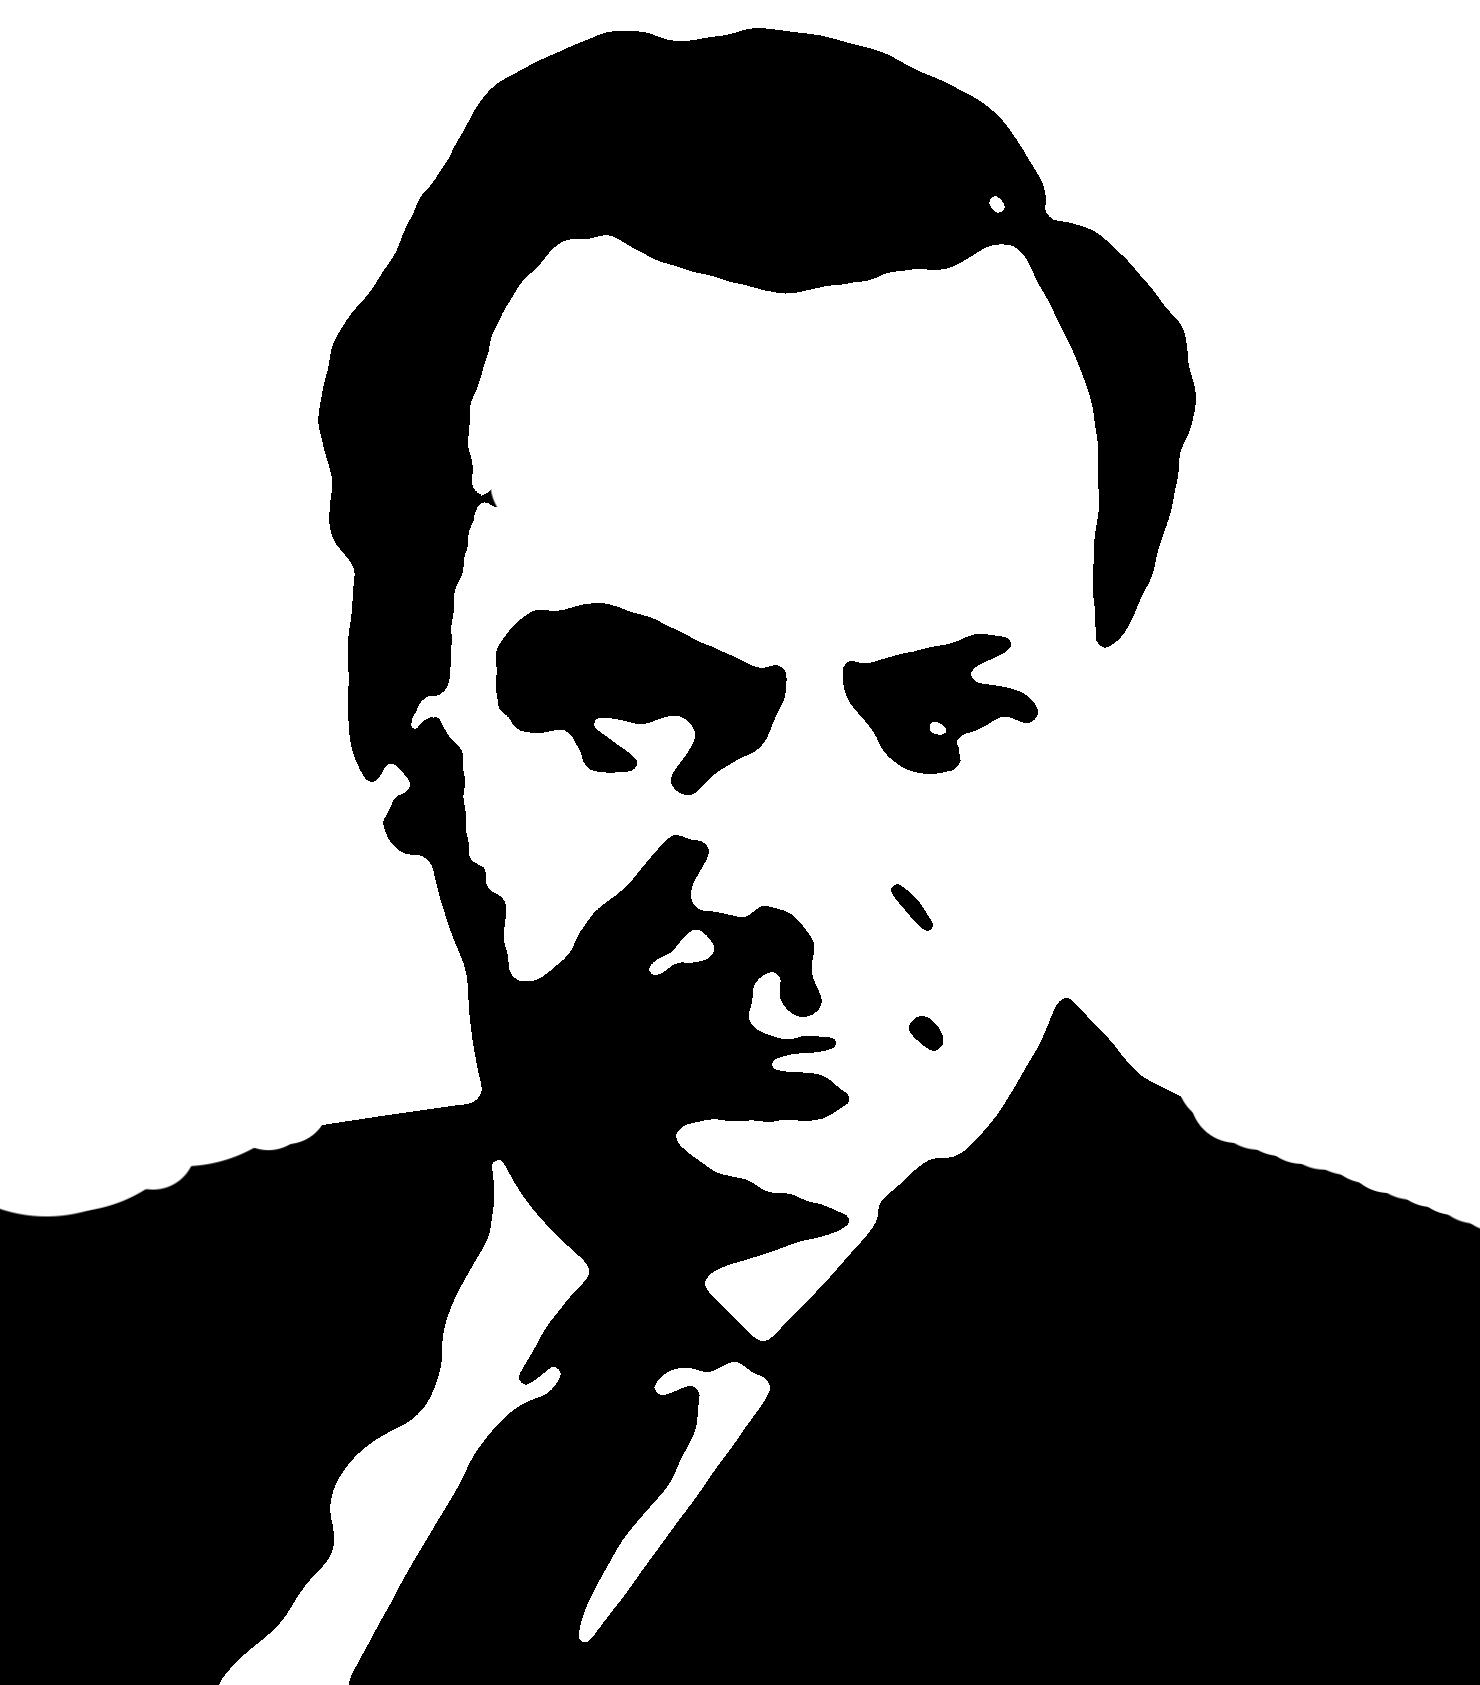
\includegraphics[height=4cm]{figures/feynman.png}
	\caption{这是一个测试: Dr. Feynman}\label{fig:feynman}
\end{figure}
\end{Verbatim}
\begin{figure}[!h]
	\centering
	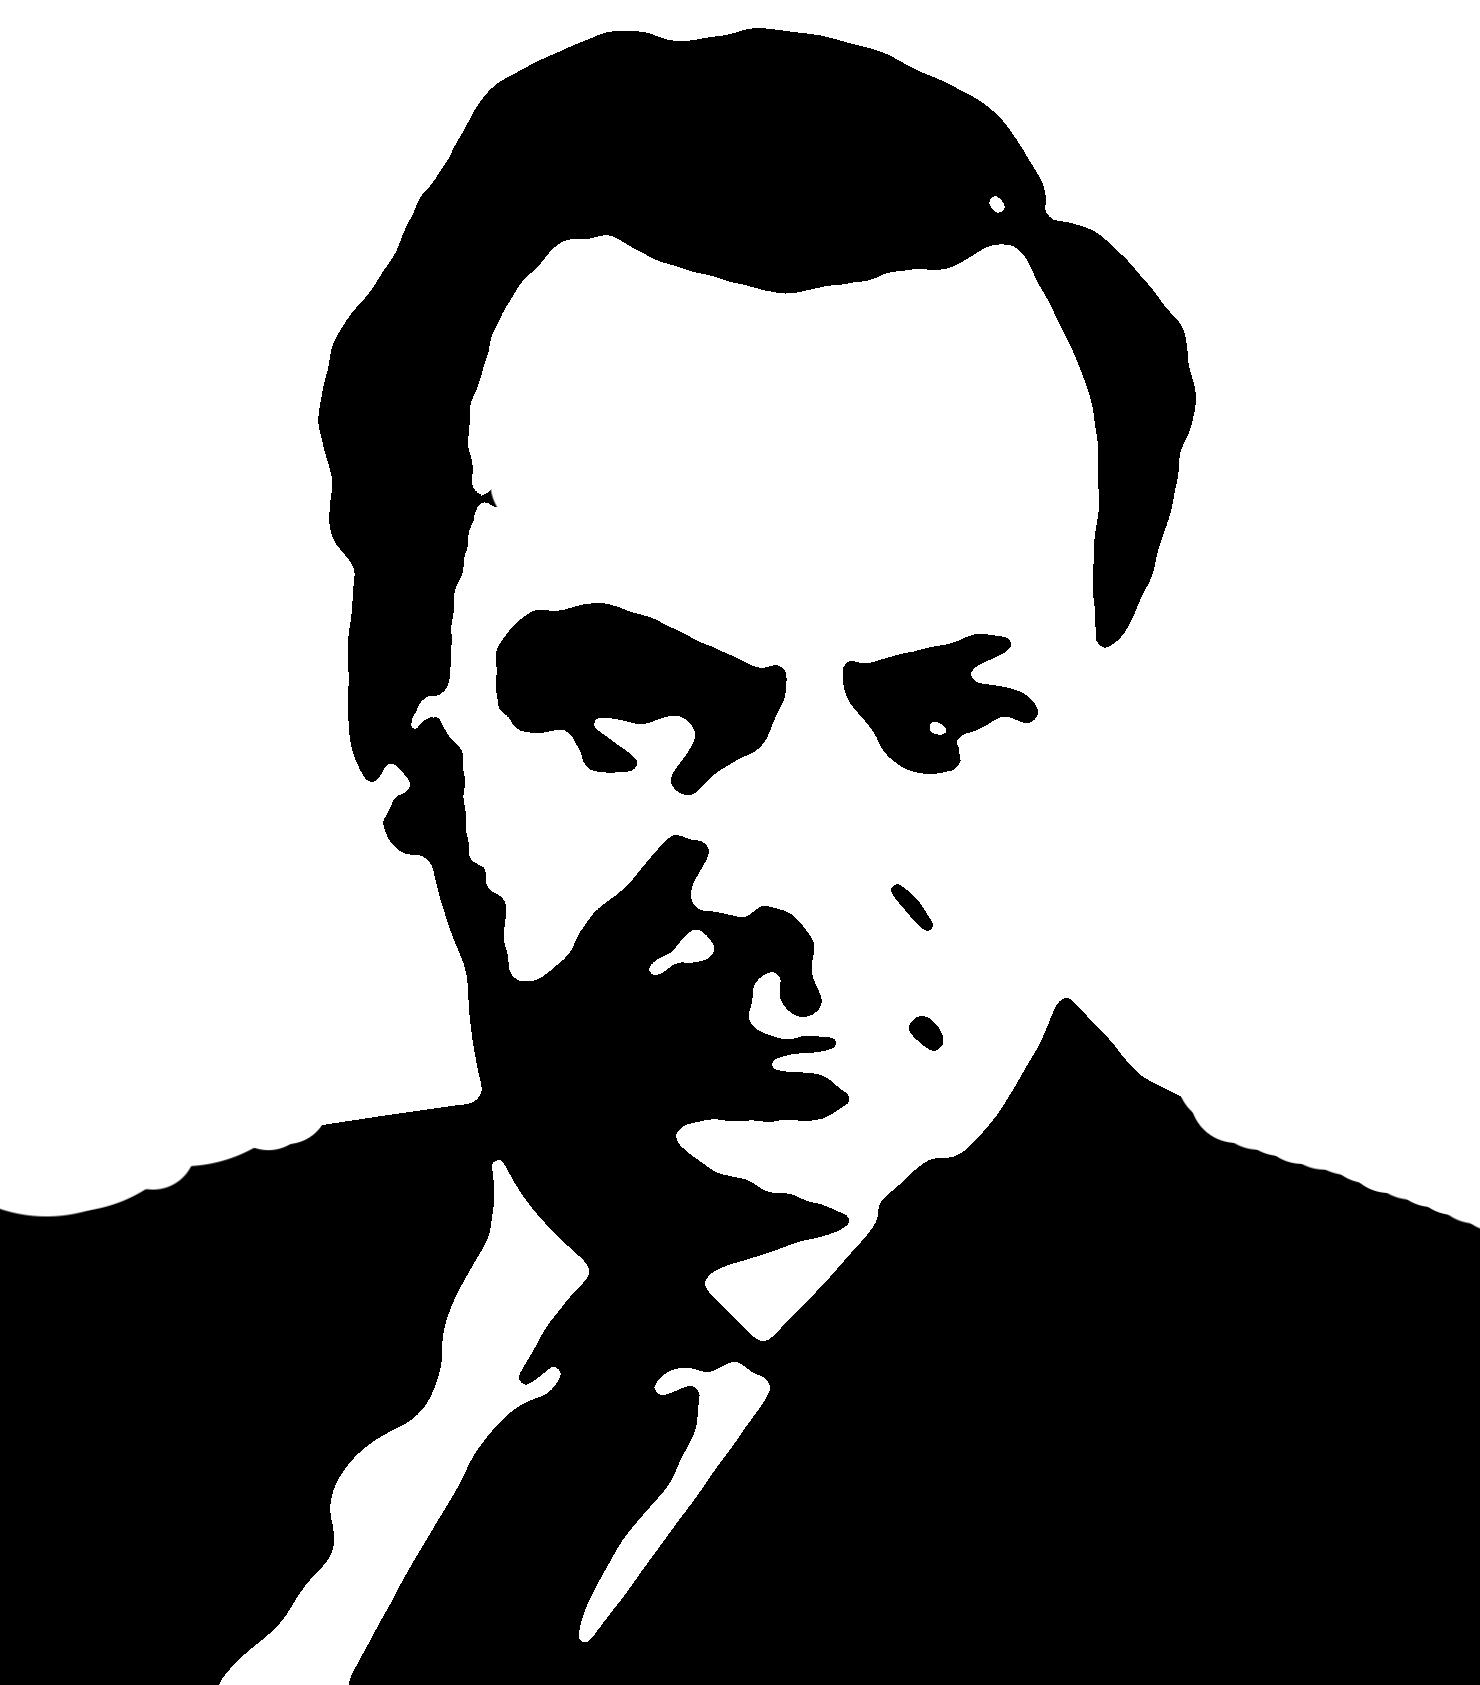
\includegraphics[height=4cm,angle=45]{figures/feynman.png}
	\caption{这是一个测试: Dr. Feynman}\label{fig:feynman}
\end{figure}
现在你应该自己就可以看懂很多代码,这跟刚才的插入表格很相似。需要注意的有 \verb|[!h]| 是为了令图片强制插入此处 \verb|h|=here,否则在浮动体 figure 环境中,可能会因为版式优化自动插到某页的顶部或者底部等。其实 LaTeX 的排版相当智能,只要将标题和标签做好,去掉 \verb|[!h]| 完全让它去排也并非不可。\verb|\includegraphics| 是插图指令也是显而易见,\emph{中括号} \verb|[]| 内指定图片的高度和角度,\emph{大括号} \verb|{}| 内是图片存放的路径。

还有一种方式通过居中环境插入没有标题的图片。之前命令 \verb|\centering| 显而易见用来居中,这里 center 自然也是居中环境:
\begin{Verbatim}[frame=single]
\begin{center}
	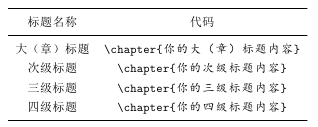
\includegraphics[height=4cm]{figures/table.png}
\end{center}
\end{Verbatim}
这样就可以产生没有标题的图片了。
\begin{center}
	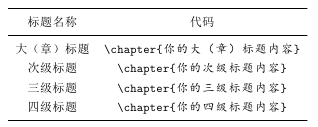
\includegraphics[height=4cm]{figures/table.png}
\end{center}
这可以用来实现在 \ref{text:table} 表格一节最后提到的技巧。不过以假乱真效果的完美与否就要看你的技巧了。

相信你现在自己也可以看着源代码学习了,其实并不难,看看源文件(比如本文档)再看看效果应该就能明白不少。这里刚就又给出了一种强调的方式,想想刚才是怎么样 \emph{emphasize}?

\subsection{列表}
列表就是列举、枚举。现在你完全可以自己看源码学会了,在第 \pageref{text:eg} 页 \ref{text:eg} 节中对操作系统的列举效果就是这样。注意,当需要有序列表时,使用 enumerate 环境即可,就像
\begin{enumerate}
	\item 张三
	\item 李四
	\item 王五
\end{enumerate}

\subsection{公式}
这是 LaTeX 最擅长的部分之一。但是因为公式在论文中的使用也不能算十分频繁,数学、计算机、物理等科系除外(其实这些专业早应该对 LaTeX 比较熟悉了),所以这里这简单说明一下如何使用公式环境。

具体来说就是行内公式使用 \verb|$公式代码$| 这样的形式,如 $E=mc^2$。而行间公式使用 \verb|$$公式代码$$|,如
$$e^{\pi i}+1=0$$
如果需要编号,可以使用 equation 环境,如:
\begin{equation}
	C=\int^B_0\log_2(1+\frac{S(f)}{N(f)})df
	\label{eqn:shannon}
\end{equation}
公式 \eqref{eqn:shannon} 就利用了标签引用这样的好处。

因为公式涉及的内容很多,而且相对专业,所以对此若有需求的话,具体细节一定请参看进一步阅读部分。

\subsection{参考文献}
参考文献部分仍然是省事的自动化生成,只不过需要自行建立~.bib 文献库。基本上所有的数据库都支持 BibTeX 格式输出,你可以自行拷贝、编辑,也可使用比如 MacTeX 发行版自带的 BibDesk 或者 JabRef 等文献管理软件进行文献库管理。这里仅进行一下演示,在需要处 \verb|\cite{标签名}| 就可以了。比如,我看了\cite{ref1},又看了\cite{ref2},还有\cite{ref3,ref4},发现世界真奇妙\cite{ref3}。这些当然都是随便找的胡扯,只是为了试试效果(而已)。

\subsection{附录}
附录并不是必须项,如果有需要就按照正文部分书写即可。不需要的话可以使用 \verb|%| 注释掉(即被注释部分不参与编译),每一行仅 \verb|%| 以后的内容均为注释内容。如果需要使用 \%,可以使用 \verb|\| 转义,即 \verb|\%|。
